{
\newcommand\myrect[5]{\draw (#1,#2) rectangle ({#1+#3},{#2+#4}) node[pos=0.5] {#5} ; }
\newcommand\minicipher[3]{
	\myrect{#1}{#2}{1}{1}{#3}
    \draw (#1+1, #2+0.3) -- (#1+1-0.15, #2+0.5) -- (#1+1, #2+1-0.3) ;
}

\begin{figure}
  \centering
  \begin{subfigure}[t]{0.45\textwidth}
    \centering
      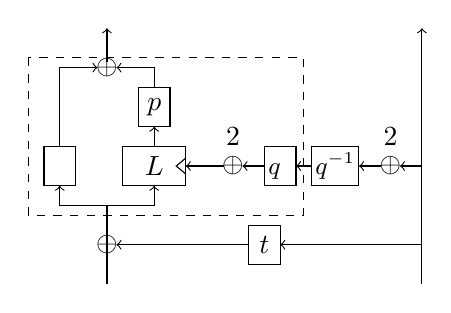
\begin{tikzpicture}[xscale=0.8, yscale=-0.5]
    	\minicipher{-0.75}{-2.5}{$L$}
    	\myrect{1.25}{-0.5}{0.5}{1}{$t$}
    	\myrect{-2}{-2.5}{0.5}{1}{$\inv$}
    	\myrect{-0.5}{-4}{0.5}{1}{$p$}
    	%\myrect{-1.375}{-6.5}{0.75}{1}{\small $p^{-1}$}
    
    	% right parallel
    	\draw [->] (4,1) -- (4,-5.5);
    
        % left bot to L and I
        \draw [->] (-1,1) -- (-1,-1) -- (-0.25,-1) -- (-0.25,-1.5);
        \draw [->]             (-1,-1) -- (-1.75,-1) -- (-1.75,-1.5);
    
    	% L to p
        \draw [->] (-0.25,-2.5) -- (-0.25,-3);
    
    	% I and p to top
        \draw [->] (-1.75,-2.5) -- (-1.75,-4.5) -- (-1.15,-4.5);
        \draw [->] (-0.25,-4) -- (-0.25,-4.5) -- (-0.85,-4.5);
    
    	% xor t
    	\draw (-1.0,-4.5) node[inner sep=0](xor){$\oplus$} ;
    
    	% xor to p^-1
    	\draw [->] (-1.0,-4.65) -- (-1.0,-5.5);
    
    	% p^-1 to top
    	%\draw [->] (-1.0,-6.5) -- (-1.0,-7.5);
    
    	% xor 2 q q^{-1} xor 2
    	\draw (1,-2) node[inner sep=0](xor){$\oplus$} ;
    	\draw (1,-2.75) node[inner sep=0](xor){2} ;
    	\myrect{1.5}{-2.5}{0.5}{1}{\small $q^{\color{white}1}$}
    	\myrect{2.25}{-2.5}{0.75}{1}{\small $q^{-1}$}
    	\draw (3.5,-2) node[inner sep=0](xor){$\oplus$} ;
    	\draw (3.5,-2.75) node[inner sep=0](xor){2} ;
    
    	% right to L key
    	\draw [->] (4,-2) -- (3.65,-2);
    	\draw [->] (3.35,-2) -- (3,-2);
    	\draw [->] (2.25,-2) -- (2,-2);
    	\draw [->] (1.5,-2) -- (1.15,-2);
    	\draw [->] (0.85,-2) -- (0.25,-2);
    
    	% right to t
    	\draw [->] (4,0) -- (1.75,0);
    	% t to xor
    	\draw [->] (1.25,0) -- (-0.85,0);
    	\draw (-1.0,0) node[inner sep=0](xor){$\oplus$} ;
    	
    	% dots
	    \draw [dashed] (-2.25,-4.75) rectangle (2.125,-0.75);
      \end{tikzpicture}
        \FigDef{simplify-pl-a}{Using $k' = q(k)\oplus 2$.}
  \end{subfigure}
  \hspace{0.2cm}
  \begin{subfigure}[t]{0.45\textwidth}
    \centering
      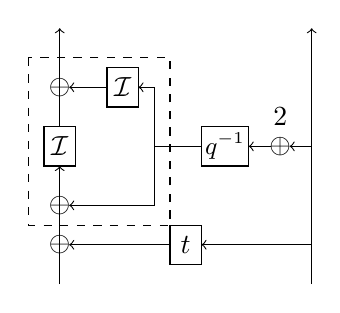
\begin{tikzpicture}[xscale=0.8, yscale=-0.5]
    	\myrect{0.75}{-0.5}{0.5}{1}{$t$}
    	\myrect{-1.25}{-3}{0.5}{1}{$\mathcal{I}$}
    	\myrect{-0.25}{-4.5}{0.5}{1}{$\mathcal{I}$}
    	%\myrect{-1.375}{-6.5}{0.75}{1}{\small $p^{-1}$}
    
    	% right parallel
    	\draw [->] (3,1) -- (3,-5.5);
    
        % left bot to I
        \draw [->] (-1,1) -- (-1,-2);
    
    	% I to p^{-1}
    	\draw [->] (-1,-3) -- (-1,-5.5);
    
    	% xor top
    	\draw (-1.0,-4) node[inner sep=0](xor){$\oplus$} ;
    
    	% p^-1 to top
    	%\draw [->] (-1.0,-6.5) -- (-1.0,-7.5);
    
    	% xor 2 q q^{-1} xor 2
    	\myrect{1.25}{-3}{0.75}{1}{\small $q^{-1}$}
    	\draw (2.5,-2.5) node[inner sep=0](xor){$\oplus$} ;
    	\draw (2.5,-3.25) node[inner sep=0](xor){2} ;
    
    	% xor riight key before I
    	\draw (-1,-1) node[inner sep=0](xor){$\oplus$} ;
    
    	% right to L key
    	\draw [->] (3,-2.5) -- (2.65,-2.5);
    	\draw [->] (2.35,-2.5) -- (2,-2.5);
    	\draw [->] (1.25,-2.5) -- (0.5,-2.5) -- (0.5,-4) -- (0.25,-4);
    	\draw [->] (-0.25,-4) -- (-0.85,-4);
    	\draw [->]                (0.5,-2.5) -- (0.5,-1) -- (-0.85,-1);
    
    	% right to t
    	\draw [->] (3,0) -- (1.25,0);
    	% t to xor
    	\draw [->] (0.75,0) -- (-0.85,0);
    	\draw (-1.0,0) node[inner sep=0](xor){$\oplus$} ;
    
    	% dots
    	\draw [dashed] (-1.5,-4.75) rectangle (0.75 ,-0.5);
      \end{tikzpicture}
    \FigDef{simplify-pl-b}{Using \EqRef{pinvTinv}.}
  \end{subfigure}
  \FigDef{simplify-pl}{Simplifying $p \circ L$ (and $p^{-1}\circ T'^{-1}$). The dashed area corresponds to the application of \EqRef{pinvTinv}.}
\end{figure}
}